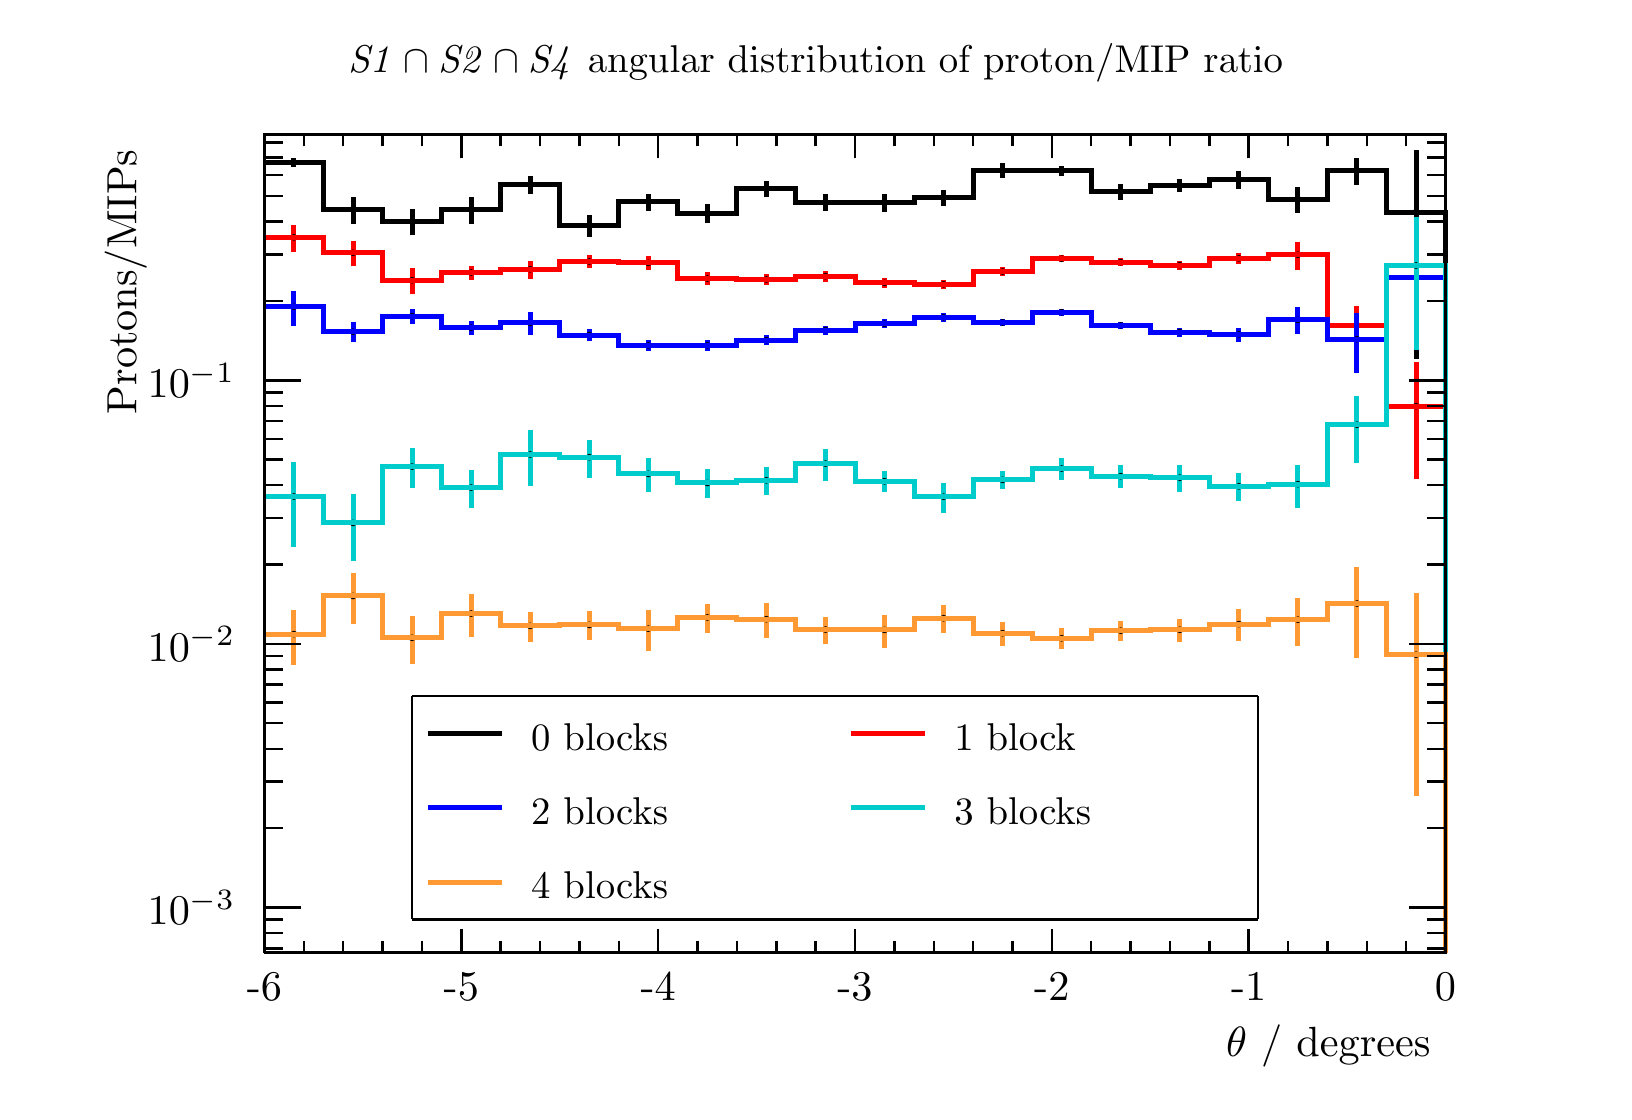
\begin{tikzpicture}
\pgfdeclareplotmark{cross} {
\pgfpathmoveto{\pgfpoint{-0.3\pgfplotmarksize}{\pgfplotmarksize}}
\pgfpathlineto{\pgfpoint{+0.3\pgfplotmarksize}{\pgfplotmarksize}}
\pgfpathlineto{\pgfpoint{+0.3\pgfplotmarksize}{0.3\pgfplotmarksize}}
\pgfpathlineto{\pgfpoint{+1\pgfplotmarksize}{0.3\pgfplotmarksize}}
\pgfpathlineto{\pgfpoint{+1\pgfplotmarksize}{-0.3\pgfplotmarksize}}
\pgfpathlineto{\pgfpoint{+0.3\pgfplotmarksize}{-0.3\pgfplotmarksize}}
\pgfpathlineto{\pgfpoint{+0.3\pgfplotmarksize}{-1.\pgfplotmarksize}}
\pgfpathlineto{\pgfpoint{-0.3\pgfplotmarksize}{-1.\pgfplotmarksize}}
\pgfpathlineto{\pgfpoint{-0.3\pgfplotmarksize}{-0.3\pgfplotmarksize}}
\pgfpathlineto{\pgfpoint{-1.\pgfplotmarksize}{-0.3\pgfplotmarksize}}
\pgfpathlineto{\pgfpoint{-1.\pgfplotmarksize}{0.3\pgfplotmarksize}}
\pgfpathlineto{\pgfpoint{-0.3\pgfplotmarksize}{0.3\pgfplotmarksize}}
\pgfpathclose
\pgfusepathqstroke
}
\pgfdeclareplotmark{cross*} {
\pgfpathmoveto{\pgfpoint{-0.3\pgfplotmarksize}{\pgfplotmarksize}}
\pgfpathlineto{\pgfpoint{+0.3\pgfplotmarksize}{\pgfplotmarksize}}
\pgfpathlineto{\pgfpoint{+0.3\pgfplotmarksize}{0.3\pgfplotmarksize}}
\pgfpathlineto{\pgfpoint{+1\pgfplotmarksize}{0.3\pgfplotmarksize}}
\pgfpathlineto{\pgfpoint{+1\pgfplotmarksize}{-0.3\pgfplotmarksize}}
\pgfpathlineto{\pgfpoint{+0.3\pgfplotmarksize}{-0.3\pgfplotmarksize}}
\pgfpathlineto{\pgfpoint{+0.3\pgfplotmarksize}{-1.\pgfplotmarksize}}
\pgfpathlineto{\pgfpoint{-0.3\pgfplotmarksize}{-1.\pgfplotmarksize}}
\pgfpathlineto{\pgfpoint{-0.3\pgfplotmarksize}{-0.3\pgfplotmarksize}}
\pgfpathlineto{\pgfpoint{-1.\pgfplotmarksize}{-0.3\pgfplotmarksize}}
\pgfpathlineto{\pgfpoint{-1.\pgfplotmarksize}{0.3\pgfplotmarksize}}
\pgfpathlineto{\pgfpoint{-0.3\pgfplotmarksize}{0.3\pgfplotmarksize}}
\pgfpathclose
\pgfusepathqfillstroke
}
\pgfdeclareplotmark{newstar} {
\pgfpathmoveto{\pgfqpoint{0pt}{\pgfplotmarksize}}
\pgfpathlineto{\pgfqpointpolar{44}{0.5\pgfplotmarksize}}
\pgfpathlineto{\pgfqpointpolar{18}{\pgfplotmarksize}}
\pgfpathlineto{\pgfqpointpolar{-20}{0.5\pgfplotmarksize}}
\pgfpathlineto{\pgfqpointpolar{-54}{\pgfplotmarksize}}
\pgfpathlineto{\pgfqpointpolar{-90}{0.5\pgfplotmarksize}}
\pgfpathlineto{\pgfqpointpolar{234}{\pgfplotmarksize}}
\pgfpathlineto{\pgfqpointpolar{198}{0.5\pgfplotmarksize}}
\pgfpathlineto{\pgfqpointpolar{162}{\pgfplotmarksize}}
\pgfpathlineto{\pgfqpointpolar{134}{0.5\pgfplotmarksize}}
\pgfpathclose
\pgfusepathqstroke
}
\pgfdeclareplotmark{newstar*} {
\pgfpathmoveto{\pgfqpoint{0pt}{\pgfplotmarksize}}
\pgfpathlineto{\pgfqpointpolar{44}{0.5\pgfplotmarksize}}
\pgfpathlineto{\pgfqpointpolar{18}{\pgfplotmarksize}}
\pgfpathlineto{\pgfqpointpolar{-20}{0.5\pgfplotmarksize}}
\pgfpathlineto{\pgfqpointpolar{-54}{\pgfplotmarksize}}
\pgfpathlineto{\pgfqpointpolar{-90}{0.5\pgfplotmarksize}}
\pgfpathlineto{\pgfqpointpolar{234}{\pgfplotmarksize}}
\pgfpathlineto{\pgfqpointpolar{198}{0.5\pgfplotmarksize}}
\pgfpathlineto{\pgfqpointpolar{162}{\pgfplotmarksize}}
\pgfpathlineto{\pgfqpointpolar{134}{0.5\pgfplotmarksize}}
\pgfpathclose
\pgfusepathqfillstroke
}
\definecolor{c}{rgb}{1,1,1};
\draw [color=c, fill=c] (0,0) rectangle (20,13.4957);
\draw [color=c, fill=c] (3,1.75444) rectangle (18,12.1461);
\definecolor{c}{rgb}{0,0,0};
\draw [c,line width=0.9] (3,1.75444) -- (3,12.1461) -- (18,12.1461) -- (18,1.75444) -- (3,1.75444);
\definecolor{c}{rgb}{1,1,1};
\draw [color=c, fill=c] (3,1.75444) rectangle (18,12.1461);
\definecolor{c}{rgb}{0,0,0};
\draw [c,line width=0.9] (3,1.75444) -- (3,12.1461) -- (18,12.1461) -- (18,1.75444) -- (3,1.75444);
\draw [c,line width=0.9] (3,1.75444) -- (3.75,1.75444) -- (3.75,1.75444) -- (4.5,1.75444) -- (4.5,1.75444) -- (5.25,1.75444) -- (5.25,1.75444) -- (6,1.75444) -- (6,1.75444) -- (6.75,1.75444) -- (6.75,1.75444) -- (7.5,1.75444) -- (7.5,1.75444) --
 (8.25,1.75444) -- (8.25,1.75444) -- (9,1.75444) -- (9,1.75444) -- (9.75,1.75444) -- (9.75,1.75444) -- (10.5,1.75444) -- (10.5,1.75444) -- (11.25,1.75444) -- (11.25,1.75444) -- (12,1.75444) -- (12,1.75444) -- (12.75,1.75444) -- (12.75,1.75444) --
 (13.5,1.75444) -- (13.5,1.75444) -- (14.25,1.75444) -- (14.25,1.75444) -- (15,1.75444) -- (15,1.75444) -- (15.75,1.75444) -- (15.75,1.75444) -- (16.5,1.75444) -- (16.5,1.75444) -- (17.25,1.75444) -- (17.25,1.75444) -- (18,1.75444) -- (18,1.75444);
\draw [c,line width=0.9] (3,1.75444) -- (18,1.75444);
\draw [c,line width=0.9] (3,2.05809) -- (3,1.75444);
\draw [c,line width=0.9] (3.5,1.90627) -- (3.5,1.75444);
\draw [c,line width=0.9] (4,1.90627) -- (4,1.75444);
\draw [c,line width=0.9] (4.5,1.90627) -- (4.5,1.75444);
\draw [c,line width=0.9] (5,1.90627) -- (5,1.75444);
\draw [c,line width=0.9] (5.5,2.05809) -- (5.5,1.75444);
\draw [c,line width=0.9] (6,1.90627) -- (6,1.75444);
\draw [c,line width=0.9] (6.5,1.90627) -- (6.5,1.75444);
\draw [c,line width=0.9] (7,1.90627) -- (7,1.75444);
\draw [c,line width=0.9] (7.5,1.90627) -- (7.5,1.75444);
\draw [c,line width=0.9] (8,2.05809) -- (8,1.75444);
\draw [c,line width=0.9] (8.5,1.90627) -- (8.5,1.75444);
\draw [c,line width=0.9] (9,1.90627) -- (9,1.75444);
\draw [c,line width=0.9] (9.5,1.90627) -- (9.5,1.75444);
\draw [c,line width=0.9] (10,1.90627) -- (10,1.75444);
\draw [c,line width=0.9] (10.5,2.05809) -- (10.5,1.75444);
\draw [c,line width=0.9] (11,1.90627) -- (11,1.75444);
\draw [c,line width=0.9] (11.5,1.90627) -- (11.5,1.75444);
\draw [c,line width=0.9] (12,1.90627) -- (12,1.75444);
\draw [c,line width=0.9] (12.5,1.90627) -- (12.5,1.75444);
\draw [c,line width=0.9] (13,2.05809) -- (13,1.75444);
\draw [c,line width=0.9] (13.5,1.90627) -- (13.5,1.75444);
\draw [c,line width=0.9] (14,1.90627) -- (14,1.75444);
\draw [c,line width=0.9] (14.5,1.90627) -- (14.5,1.75444);
\draw [c,line width=0.9] (15,1.90627) -- (15,1.75444);
\draw [c,line width=0.9] (15.5,2.05809) -- (15.5,1.75444);
\draw [c,line width=0.9] (16,1.90627) -- (16,1.75444);
\draw [c,line width=0.9] (16.5,1.90627) -- (16.5,1.75444);
\draw [c,line width=0.9] (17,1.90627) -- (17,1.75444);
\draw [c,line width=0.9] (17.5,1.90627) -- (17.5,1.75444);
\draw [c,line width=0.9] (18,2.05809) -- (18,1.75444);
\draw [anchor=base] (3,1.14713) node[scale=1.52731, color=c, rotate=0]{-6};
\draw [anchor=base] (5.5,1.14713) node[scale=1.52731, color=c, rotate=0]{-5};
\draw [anchor=base] (8,1.14713) node[scale=1.52731, color=c, rotate=0]{-4};
\draw [anchor=base] (10.5,1.14713) node[scale=1.52731, color=c, rotate=0]{-3};
\draw [anchor=base] (13,1.14713) node[scale=1.52731, color=c, rotate=0]{-2};
\draw [anchor=base] (15.5,1.14713) node[scale=1.52731, color=c, rotate=0]{-1};
\draw [anchor=base] (18,1.14713) node[scale=1.52731, color=c, rotate=0]{0};
\draw [anchor= east] (18,0.566819) node[scale=1.52731, color=c, rotate=0]{$ \theta$ / degrees};
\draw [c,line width=0.9] (3,12.1461) -- (18,12.1461);
\draw [c,line width=0.9] (3,11.8425) -- (3,12.1461);
\draw [c,line width=0.9] (3.5,11.9943) -- (3.5,12.1461);
\draw [c,line width=0.9] (4,11.9943) -- (4,12.1461);
\draw [c,line width=0.9] (4.5,11.9943) -- (4.5,12.1461);
\draw [c,line width=0.9] (5,11.9943) -- (5,12.1461);
\draw [c,line width=0.9] (5.5,11.8425) -- (5.5,12.1461);
\draw [c,line width=0.9] (6,11.9943) -- (6,12.1461);
\draw [c,line width=0.9] (6.5,11.9943) -- (6.5,12.1461);
\draw [c,line width=0.9] (7,11.9943) -- (7,12.1461);
\draw [c,line width=0.9] (7.5,11.9943) -- (7.5,12.1461);
\draw [c,line width=0.9] (8,11.8425) -- (8,12.1461);
\draw [c,line width=0.9] (8.5,11.9943) -- (8.5,12.1461);
\draw [c,line width=0.9] (9,11.9943) -- (9,12.1461);
\draw [c,line width=0.9] (9.5,11.9943) -- (9.5,12.1461);
\draw [c,line width=0.9] (10,11.9943) -- (10,12.1461);
\draw [c,line width=0.9] (10.5,11.8425) -- (10.5,12.1461);
\draw [c,line width=0.9] (11,11.9943) -- (11,12.1461);
\draw [c,line width=0.9] (11.5,11.9943) -- (11.5,12.1461);
\draw [c,line width=0.9] (12,11.9943) -- (12,12.1461);
\draw [c,line width=0.9] (12.5,11.9943) -- (12.5,12.1461);
\draw [c,line width=0.9] (13,11.8425) -- (13,12.1461);
\draw [c,line width=0.9] (13.5,11.9943) -- (13.5,12.1461);
\draw [c,line width=0.9] (14,11.9943) -- (14,12.1461);
\draw [c,line width=0.9] (14.5,11.9943) -- (14.5,12.1461);
\draw [c,line width=0.9] (15,11.9943) -- (15,12.1461);
\draw [c,line width=0.9] (15.5,11.8425) -- (15.5,12.1461);
\draw [c,line width=0.9] (16,11.9943) -- (16,12.1461);
\draw [c,line width=0.9] (16.5,11.9943) -- (16.5,12.1461);
\draw [c,line width=0.9] (17,11.9943) -- (17,12.1461);
\draw [c,line width=0.9] (17.5,11.9943) -- (17.5,12.1461);
\draw [c,line width=0.9] (18,11.8425) -- (18,12.1461);
\draw [c,line width=0.9] (3,1.75444) -- (3,12.1461);
\draw [c,line width=0.9] (3.231,1.81119) -- (3,1.81119);
\draw [c,line width=0.9] (3.231,2.00531) -- (3,2.00531);
\draw [c,line width=0.9] (3.231,2.17652) -- (3,2.17652);
\draw [c,line width=0.9] (3.462,2.32968) -- (3,2.32968);
\draw [anchor= east] (2.82,2.32968) node[scale=1.52731, color=c, rotate=0]{$10^{-3}$};
\draw [c,line width=0.9] (3.231,3.3373) -- (3,3.3373);
\draw [c,line width=0.9] (3.231,3.92671) -- (3,3.92671);
\draw [c,line width=0.9] (3.231,4.34491) -- (3,4.34491);
\draw [c,line width=0.9] (3.231,4.66929) -- (3,4.66929);
\draw [c,line width=0.9] (3.231,4.93432) -- (3,4.93432);
\draw [c,line width=0.9] (3.231,5.15841) -- (3,5.15841);
\draw [c,line width=0.9] (3.231,5.35252) -- (3,5.35252);
\draw [c,line width=0.9] (3.231,5.52374) -- (3,5.52374);
\draw [c,line width=0.9] (3.462,5.6769) -- (3,5.6769);
\draw [anchor= east] (2.82,5.6769) node[scale=1.52731, color=c, rotate=0]{$10^{-2}$};
\draw [c,line width=0.9] (3.231,6.68451) -- (3,6.68451);
\draw [c,line width=0.9] (3.231,7.27392) -- (3,7.27392);
\draw [c,line width=0.9] (3.231,7.69212) -- (3,7.69212);
\draw [c,line width=0.9] (3.231,8.0165) -- (3,8.0165);
\draw [c,line width=0.9] (3.231,8.28153) -- (3,8.28153);
\draw [c,line width=0.9] (3.231,8.50562) -- (3,8.50562);
\draw [c,line width=0.9] (3.231,8.69973) -- (3,8.69973);
\draw [c,line width=0.9] (3.231,8.87095) -- (3,8.87095);
\draw [c,line width=0.9] (3.462,9.02411) -- (3,9.02411);
\draw [anchor= east] (2.82,9.02411) node[scale=1.52731, color=c, rotate=0]{$10^{-1}$};
\draw [c,line width=0.9] (3.231,10.0317) -- (3,10.0317);
\draw [c,line width=0.9] (3.231,10.6211) -- (3,10.6211);
\draw [c,line width=0.9] (3.231,11.0393) -- (3,11.0393);
\draw [c,line width=0.9] (3.231,11.3637) -- (3,11.3637);
\draw [c,line width=0.9] (3.231,11.6287) -- (3,11.6287);
\draw [c,line width=0.9] (3.231,11.8528) -- (3,11.8528);
\draw [c,line width=0.9] (3.231,12.0469) -- (3,12.0469);
\draw [anchor= east] (1.24,12.1461) node[scale=1.52731, color=c, rotate=90]{ Protons/MIPs};
\draw [c,line width=0.9] (18,1.75444) -- (18,12.1461);
\draw [c,line width=0.9] (17.769,1.81119) -- (18,1.81119);
\draw [c,line width=0.9] (17.769,2.00531) -- (18,2.00531);
\draw [c,line width=0.9] (17.769,2.17652) -- (18,2.17652);
\draw [c,line width=0.9] (17.538,2.32968) -- (18,2.32968);
\draw [c,line width=0.9] (17.769,3.3373) -- (18,3.3373);
\draw [c,line width=0.9] (17.769,3.92671) -- (18,3.92671);
\draw [c,line width=0.9] (17.769,4.34491) -- (18,4.34491);
\draw [c,line width=0.9] (17.769,4.66929) -- (18,4.66929);
\draw [c,line width=0.9] (17.769,4.93432) -- (18,4.93432);
\draw [c,line width=0.9] (17.769,5.15841) -- (18,5.15841);
\draw [c,line width=0.9] (17.769,5.35252) -- (18,5.35252);
\draw [c,line width=0.9] (17.769,5.52374) -- (18,5.52374);
\draw [c,line width=0.9] (17.538,5.6769) -- (18,5.6769);
\draw [c,line width=0.9] (17.769,6.68451) -- (18,6.68451);
\draw [c,line width=0.9] (17.769,7.27392) -- (18,7.27392);
\draw [c,line width=0.9] (17.769,7.69212) -- (18,7.69212);
\draw [c,line width=0.9] (17.769,8.0165) -- (18,8.0165);
\draw [c,line width=0.9] (17.769,8.28153) -- (18,8.28153);
\draw [c,line width=0.9] (17.769,8.50562) -- (18,8.50562);
\draw [c,line width=0.9] (17.769,8.69973) -- (18,8.69973);
\draw [c,line width=0.9] (17.769,8.87095) -- (18,8.87095);
\draw [c,line width=0.9] (17.538,9.02411) -- (18,9.02411);
\draw [c,line width=0.9] (17.769,10.0317) -- (18,10.0317);
\draw [c,line width=0.9] (17.769,10.6211) -- (18,10.6211);
\draw [c,line width=0.9] (17.769,11.0393) -- (18,11.0393);
\draw [c,line width=0.9] (17.769,11.3637) -- (18,11.3637);
\draw [c,line width=0.9] (17.769,11.6287) -- (18,11.6287);
\draw [c,line width=0.9] (17.769,11.8528) -- (18,11.8528);
\draw [c,line width=0.9] (17.769,12.0469) -- (18,12.0469);
\draw [c,line width=1.8] (3.375,11.7286) -- (3.375,11.7905);
\draw [c,line width=1.8] (3.375,11.7905) -- (3.375,11.8499);
\foreach \P in {(3.375,11.7905)}{\draw[mark options={color=c,fill=c},mark size=2.402402pt,mark=*,mark size=1pt] plot coordinates {\P};}
\draw [c,line width=1.8] (4.125,11.011) -- (4.125,11.1945);
\draw [c,line width=1.8] (4.125,11.1945) -- (4.125,11.3574);
\foreach \P in {(4.125,11.1945)}{\draw[mark options={color=c,fill=c},mark size=2.402402pt,mark=*,mark size=1pt] plot coordinates {\P};}
\draw [c,line width=1.8] (4.875,10.8641) -- (4.875,11.0421);
\draw [c,line width=1.8] (4.875,11.0421) -- (4.875,11.2007);
\foreach \P in {(4.875,11.0421)}{\draw[mark options={color=c,fill=c},mark size=2.402402pt,mark=*,mark size=1pt] plot coordinates {\P};}
\draw [c,line width=1.8] (5.625,11.0063) -- (5.625,11.1929);
\draw [c,line width=1.8] (5.625,11.1929) -- (5.625,11.3583);
\foreach \P in {(5.625,11.1929)}{\draw[mark options={color=c,fill=c},mark size=2.402402pt,mark=*,mark size=1pt] plot coordinates {\P};}
\draw [c,line width=1.8] (6.375,11.3864) -- (6.375,11.5075);
\draw [c,line width=1.8] (6.375,11.5075) -- (6.375,11.6193);
\foreach \P in {(6.375,11.5075)}{\draw[mark options={color=c,fill=c},mark size=2.402402pt,mark=*,mark size=1pt] plot coordinates {\P};}
\draw [c,line width=1.8] (7.125,10.8457) -- (7.125,10.9898);
\draw [c,line width=1.8] (7.125,10.9898) -- (7.125,11.121);
\foreach \P in {(7.125,10.9898)}{\draw[mark options={color=c,fill=c},mark size=2.402402pt,mark=*,mark size=1pt] plot coordinates {\P};}
\draw [c,line width=1.8] (7.875,11.1787) -- (7.875,11.2895);
\draw [c,line width=1.8] (7.875,11.2895) -- (7.875,11.3925);
\foreach \P in {(7.875,11.2895)}{\draw[mark options={color=c,fill=c},mark size=2.402402pt,mark=*,mark size=1pt] plot coordinates {\P};}
\draw [c,line width=1.8] (8.625,11.016) -- (8.625,11.1471);
\draw [c,line width=1.8] (8.625,11.1471) -- (8.625,11.2673);
\foreach \P in {(8.625,11.1471)}{\draw[mark options={color=c,fill=c},mark size=2.402402pt,mark=*,mark size=1pt] plot coordinates {\P};}
\draw [c,line width=1.8] (9.375,11.3486) -- (9.375,11.4549);
\draw [c,line width=1.8] (9.375,11.4549) -- (9.375,11.554);
\foreach \P in {(9.375,11.4549)}{\draw[mark options={color=c,fill=c},mark size=2.402402pt,mark=*,mark size=1pt] plot coordinates {\P};}
\draw [c,line width=1.8] (10.125,11.1709) -- (10.125,11.2835);
\draw [c,line width=1.8] (10.125,11.2835) -- (10.125,11.388);
\foreach \P in {(10.125,11.2835)}{\draw[mark options={color=c,fill=c},mark size=2.402402pt,mark=*,mark size=1pt] plot coordinates {\P};}
\draw [c,line width=1.8] (10.875,11.1574) -- (10.875,11.2802);
\draw [c,line width=1.8] (10.875,11.2802) -- (10.875,11.3935);
\foreach \P in {(10.875,11.2802)}{\draw[mark options={color=c,fill=c},mark size=2.402402pt,mark=*,mark size=1pt] plot coordinates {\P};}
\draw [c,line width=1.8] (11.625,11.2428) -- (11.625,11.342);
\draw [c,line width=1.8] (11.625,11.342) -- (11.625,11.4348);
\foreach \P in {(11.625,11.342)}{\draw[mark options={color=c,fill=c},mark size=2.402402pt,mark=*,mark size=1pt] plot coordinates {\P};}
\draw [c,line width=1.8] (12.375,11.5967) -- (12.375,11.6916);
\draw [c,line width=1.8] (12.375,11.6916) -- (12.375,11.7807);
\foreach \P in {(12.375,11.6916)}{\draw[mark options={color=c,fill=c},mark size=2.402402pt,mark=*,mark size=1pt] plot coordinates {\P};}
\draw [c,line width=1.8] (13.125,11.6131) -- (13.125,11.6836);
\draw [c,line width=1.8] (13.125,11.6836) -- (13.125,11.7508);
\foreach \P in {(13.125,11.6836)}{\draw[mark options={color=c,fill=c},mark size=2.402402pt,mark=*,mark size=1pt] plot coordinates {\P};}
\draw [c,line width=1.8] (13.875,11.3187) -- (13.875,11.4194);
\draw [c,line width=1.8] (13.875,11.4194) -- (13.875,11.5135);
\foreach \P in {(13.875,11.4194)}{\draw[mark options={color=c,fill=c},mark size=2.402402pt,mark=*,mark size=1pt] plot coordinates {\P};}
\draw [c,line width=1.8] (14.625,11.4104) -- (14.625,11.5007);
\draw [c,line width=1.8] (14.625,11.5007) -- (14.625,11.5857);
\foreach \P in {(14.625,11.5007)}{\draw[mark options={color=c,fill=c},mark size=2.402402pt,mark=*,mark size=1pt] plot coordinates {\P};}
\draw [c,line width=1.8] (15.375,11.4577) -- (15.375,11.5727);
\draw [c,line width=1.8] (15.375,11.5727) -- (15.375,11.6792);
\foreach \P in {(15.375,11.5727)}{\draw[mark options={color=c,fill=c},mark size=2.402402pt,mark=*,mark size=1pt] plot coordinates {\P};}
\draw [c,line width=1.8] (16.125,11.1513) -- (16.125,11.3259);
\draw [c,line width=1.8] (16.125,11.3259) -- (16.125,11.4817);
\foreach \P in {(16.125,11.3259)}{\draw[mark options={color=c,fill=c},mark size=2.402402pt,mark=*,mark size=1pt] plot coordinates {\P};}
\draw [c,line width=1.8] (16.875,11.504) -- (16.875,11.6859);
\draw [c,line width=1.8] (16.875,11.6859) -- (16.875,11.8475);
\foreach \P in {(16.875,11.6859)}{\draw[mark options={color=c,fill=c},mark size=2.402402pt,mark=*,mark size=1pt] plot coordinates {\P};}
\draw [c,line width=1.8] (17.625,9.29325) -- (17.625,11.1604);
\draw [c,line width=1.8] (17.625,11.1604) -- (17.625,11.9515);
\foreach \P in {(17.625,11.1604)}{\draw[mark options={color=c,fill=c},mark size=2.402402pt,mark=*,mark size=1pt] plot coordinates {\P};}
\draw [c,line width=1.8] (3,11.7905) -- (3.75,11.7905) -- (3.75,11.1945) -- (4.5,11.1945) -- (4.5,11.0421) -- (5.25,11.0421) -- (5.25,11.1929) -- (6,11.1929) -- (6,11.5075) -- (6.75,11.5075) -- (6.75,10.9898) -- (7.5,10.9898) -- (7.5,11.2895) --
 (8.25,11.2895) -- (8.25,11.1471) -- (9,11.1471) -- (9,11.4549) -- (9.75,11.4549) -- (9.75,11.2835) -- (10.5,11.2835) -- (10.5,11.2802) -- (11.25,11.2802) -- (11.25,11.342) -- (12,11.342) -- (12,11.6916) -- (12.75,11.6916) -- (12.75,11.6836) --
 (13.5,11.6836) -- (13.5,11.4194) -- (14.25,11.4194) -- (14.25,11.5007) -- (15,11.5007) -- (15,11.5727) -- (15.75,11.5727) -- (15.75,11.3259) -- (16.5,11.3259) -- (16.5,11.6859) -- (17.25,11.6859) -- (17.25,11.1604) -- (18,11.1604) -- (18,1.75444);
\definecolor{c}{rgb}{1,0,0};
\draw [c,line width=1.8] (3.375,10.6566) -- (3.375,10.8395);
\draw [c,line width=1.8] (3.375,10.8395) -- (3.375,11.0019);
\definecolor{c}{rgb}{0,0,0};
\foreach \P in {(3.375,10.8395)}{\draw[mark options={color=c,fill=c},mark size=2.402402pt,mark=*,mark size=1pt] plot coordinates {\P};}
\definecolor{c}{rgb}{1,0,0};
\draw [c,line width=1.8] (4.125,10.4723) -- (4.125,10.6436);
\draw [c,line width=1.8] (4.125,10.6436) -- (4.125,10.7968);
\definecolor{c}{rgb}{0,0,0};
\foreach \P in {(4.125,10.6436)}{\draw[mark options={color=c,fill=c},mark size=2.402402pt,mark=*,mark size=1pt] plot coordinates {\P};}
\definecolor{c}{rgb}{1,0,0};
\draw [c,line width=1.8] (4.875,10.1163) -- (4.875,10.2954);
\draw [c,line width=1.8] (4.875,10.2954) -- (4.875,10.4548);
\definecolor{c}{rgb}{0,0,0};
\foreach \P in {(4.875,10.2954)}{\draw[mark options={color=c,fill=c},mark size=2.402402pt,mark=*,mark size=1pt] plot coordinates {\P};}
\definecolor{c}{rgb}{1,0,0};
\draw [c,line width=1.8] (5.625,10.3004) -- (5.625,10.3933);
\draw [c,line width=1.8] (5.625,10.3933) -- (5.625,10.4806);
\definecolor{c}{rgb}{0,0,0};
\foreach \P in {(5.625,10.3933)}{\draw[mark options={color=c,fill=c},mark size=2.402402pt,mark=*,mark size=1pt] plot coordinates {\P};}
\definecolor{c}{rgb}{1,0,0};
\draw [c,line width=1.8] (6.375,10.317) -- (6.375,10.4345);
\draw [c,line width=1.8] (6.375,10.4345) -- (6.375,10.5431);
\definecolor{c}{rgb}{0,0,0};
\foreach \P in {(6.375,10.4345)}{\draw[mark options={color=c,fill=c},mark size=2.402402pt,mark=*,mark size=1pt] plot coordinates {\P};}
\definecolor{c}{rgb}{1,0,0};
\draw [c,line width=1.8] (7.125,10.4467) -- (7.125,10.5334);
\draw [c,line width=1.8] (7.125,10.5334) -- (7.125,10.6153);
\definecolor{c}{rgb}{0,0,0};
\foreach \P in {(7.125,10.5334)}{\draw[mark options={color=c,fill=c},mark size=2.402402pt,mark=*,mark size=1pt] plot coordinates {\P};}
\definecolor{c}{rgb}{1,0,0};
\draw [c,line width=1.8] (7.875,10.4273) -- (7.875,10.5158);
\draw [c,line width=1.8] (7.875,10.5158) -- (7.875,10.5993);
\definecolor{c}{rgb}{0,0,0};
\foreach \P in {(7.875,10.5158)}{\draw[mark options={color=c,fill=c},mark size=2.402402pt,mark=*,mark size=1pt] plot coordinates {\P};}
\definecolor{c}{rgb}{1,0,0};
\draw [c,line width=1.8] (8.625,10.2337) -- (8.625,10.3167);
\draw [c,line width=1.8] (8.625,10.3167) -- (8.625,10.3952);
\definecolor{c}{rgb}{0,0,0};
\foreach \P in {(8.625,10.3167)}{\draw[mark options={color=c,fill=c},mark size=2.402402pt,mark=*,mark size=1pt] plot coordinates {\P};}
\definecolor{c}{rgb}{1,0,0};
\draw [c,line width=1.8] (9.375,10.2387) -- (9.375,10.305);
\draw [c,line width=1.8] (9.375,10.305) -- (9.375,10.3685);
\definecolor{c}{rgb}{0,0,0};
\foreach \P in {(9.375,10.305)}{\draw[mark options={color=c,fill=c},mark size=2.402402pt,mark=*,mark size=1pt] plot coordinates {\P};}
\definecolor{c}{rgb}{1,0,0};
\draw [c,line width=1.8] (10.125,10.2787) -- (10.125,10.347);
\draw [c,line width=1.8] (10.125,10.347) -- (10.125,10.4123);
\definecolor{c}{rgb}{0,0,0};
\foreach \P in {(10.125,10.347)}{\draw[mark options={color=c,fill=c},mark size=2.402402pt,mark=*,mark size=1pt] plot coordinates {\P};}
\definecolor{c}{rgb}{1,0,0};
\draw [c,line width=1.8] (10.875,10.1979) -- (10.875,10.2624);
\draw [c,line width=1.8] (10.875,10.2624) -- (10.875,10.3241);
\definecolor{c}{rgb}{0,0,0};
\foreach \P in {(10.875,10.2624)}{\draw[mark options={color=c,fill=c},mark size=2.402402pt,mark=*,mark size=1pt] plot coordinates {\P};}
\definecolor{c}{rgb}{1,0,0};
\draw [c,line width=1.8] (11.625,10.1833) -- (11.625,10.243);
\draw [c,line width=1.8] (11.625,10.243) -- (11.625,10.3003);
\definecolor{c}{rgb}{0,0,0};
\foreach \P in {(11.625,10.243)}{\draw[mark options={color=c,fill=c},mark size=2.402402pt,mark=*,mark size=1pt] plot coordinates {\P};}
\definecolor{c}{rgb}{1,0,0};
\draw [c,line width=1.8] (12.375,10.3521) -- (12.375,10.4056);
\draw [c,line width=1.8] (12.375,10.4056) -- (12.375,10.4572);
\definecolor{c}{rgb}{0,0,0};
\foreach \P in {(12.375,10.4056)}{\draw[mark options={color=c,fill=c},mark size=2.402402pt,mark=*,mark size=1pt] plot coordinates {\P};}
\definecolor{c}{rgb}{1,0,0};
\draw [c,line width=1.8] (13.125,10.5239) -- (13.125,10.5688);
\draw [c,line width=1.8] (13.125,10.5688) -- (13.125,10.6123);
\definecolor{c}{rgb}{0,0,0};
\foreach \P in {(13.125,10.5688)}{\draw[mark options={color=c,fill=c},mark size=2.402402pt,mark=*,mark size=1pt] plot coordinates {\P};}
\definecolor{c}{rgb}{1,0,0};
\draw [c,line width=1.8] (13.875,10.4749) -- (13.875,10.5252);
\draw [c,line width=1.8] (13.875,10.5252) -- (13.875,10.5738);
\definecolor{c}{rgb}{0,0,0};
\foreach \P in {(13.875,10.5252)}{\draw[mark options={color=c,fill=c},mark size=2.402402pt,mark=*,mark size=1pt] plot coordinates {\P};}
\definecolor{c}{rgb}{1,0,0};
\draw [c,line width=1.8] (14.625,10.429) -- (14.625,10.4874);
\draw [c,line width=1.8] (14.625,10.4874) -- (14.625,10.5435);
\definecolor{c}{rgb}{0,0,0};
\foreach \P in {(14.625,10.4874)}{\draw[mark options={color=c,fill=c},mark size=2.402402pt,mark=*,mark size=1pt] plot coordinates {\P};}
\definecolor{c}{rgb}{1,0,0};
\draw [c,line width=1.8] (15.375,10.4957) -- (15.375,10.5727);
\draw [c,line width=1.8] (15.375,10.5727) -- (15.375,10.6459);
\definecolor{c}{rgb}{0,0,0};
\foreach \P in {(15.375,10.5727)}{\draw[mark options={color=c,fill=c},mark size=2.402402pt,mark=*,mark size=1pt] plot coordinates {\P};}
\definecolor{c}{rgb}{1,0,0};
\draw [c,line width=1.8] (16.125,10.4296) -- (16.125,10.619);
\draw [c,line width=1.8] (16.125,10.619) -- (16.125,10.7866);
\definecolor{c}{rgb}{0,0,0};
\foreach \P in {(16.125,10.619)}{\draw[mark options={color=c,fill=c},mark size=2.402402pt,mark=*,mark size=1pt] plot coordinates {\P};}
\definecolor{c}{rgb}{1,0,0};
\draw [c,line width=1.8] (16.875,9.43238) -- (16.875,9.72304);
\draw [c,line width=1.8] (16.875,9.72304) -- (16.875,9.96515);
\definecolor{c}{rgb}{0,0,0};
\foreach \P in {(16.875,9.72304)}{\draw[mark options={color=c,fill=c},mark size=2.402402pt,mark=*,mark size=1pt] plot coordinates {\P};}
\definecolor{c}{rgb}{1,0,0};
\draw [c,line width=1.8] (17.625,7.76794) -- (17.625,8.69622);
\draw [c,line width=1.8] (17.625,8.69622) -- (17.625,9.25819);
\definecolor{c}{rgb}{0,0,0};
\foreach \P in {(17.625,8.69622)}{\draw[mark options={color=c,fill=c},mark size=2.402402pt,mark=*,mark size=1pt] plot coordinates {\P};}
\definecolor{c}{rgb}{1,0,0};
\draw [c,line width=1.8] (3,10.8395) -- (3.75,10.8395) -- (3.75,10.6436) -- (4.5,10.6436) -- (4.5,10.2954) -- (5.25,10.2954) -- (5.25,10.3933) -- (6,10.3933) -- (6,10.4345) -- (6.75,10.4345) -- (6.75,10.5334) -- (7.5,10.5334) -- (7.5,10.5158) --
 (8.25,10.5158) -- (8.25,10.3167) -- (9,10.3167) -- (9,10.305) -- (9.75,10.305) -- (9.75,10.347) -- (10.5,10.347) -- (10.5,10.2624) -- (11.25,10.2624) -- (11.25,10.243) -- (12,10.243) -- (12,10.4056) -- (12.75,10.4056) -- (12.75,10.5688) --
 (13.5,10.5688) -- (13.5,10.5252) -- (14.25,10.5252) -- (14.25,10.4874) -- (15,10.4874) -- (15,10.5727) -- (15.75,10.5727) -- (15.75,10.619) -- (16.5,10.619) -- (16.5,9.72304) -- (17.25,9.72304) -- (17.25,8.69622) -- (18,8.69622) -- (18,1.75444);
\definecolor{c}{rgb}{0,0,1};
\draw [c,line width=1.8] (3.375,9.71936) -- (3.375,9.9578);
\draw [c,line width=1.8] (3.375,9.9578) -- (3.375,10.1626);
\definecolor{c}{rgb}{0,0,0};
\foreach \P in {(3.375,9.9578)}{\draw[mark options={color=c,fill=c},mark size=2.402402pt,mark=*,mark size=1pt] plot coordinates {\P};}
\definecolor{c}{rgb}{0,0,1};
\draw [c,line width=1.8] (4.125,9.50512) -- (4.125,9.64118);
\draw [c,line width=1.8] (4.125,9.64118) -- (4.125,9.76558);
\definecolor{c}{rgb}{0,0,0};
\foreach \P in {(4.125,9.64118)}{\draw[mark options={color=c,fill=c},mark size=2.402402pt,mark=*,mark size=1pt] plot coordinates {\P};}
\definecolor{c}{rgb}{0,0,1};
\draw [c,line width=1.8] (4.875,9.73798) -- (4.875,9.83886);
\draw [c,line width=1.8] (4.875,9.83886) -- (4.875,9.93319);
\definecolor{c}{rgb}{0,0,0};
\foreach \P in {(4.875,9.83886)}{\draw[mark options={color=c,fill=c},mark size=2.402402pt,mark=*,mark size=1pt] plot coordinates {\P};}
\definecolor{c}{rgb}{0,0,1};
\draw [c,line width=1.8] (5.625,9.60133) -- (5.625,9.69315);
\draw [c,line width=1.8] (5.625,9.69315) -- (5.625,9.77951);
\definecolor{c}{rgb}{0,0,0};
\foreach \P in {(5.625,9.69315)}{\draw[mark options={color=c,fill=c},mark size=2.402402pt,mark=*,mark size=1pt] plot coordinates {\P};}
\definecolor{c}{rgb}{0,0,1};
\draw [c,line width=1.8] (6.375,9.60514) -- (6.375,9.75337);
\draw [c,line width=1.8] (6.375,9.75337) -- (6.375,9.88788);
\definecolor{c}{rgb}{0,0,0};
\foreach \P in {(6.375,9.75337)}{\draw[mark options={color=c,fill=c},mark size=2.402402pt,mark=*,mark size=1pt] plot coordinates {\P};}
\definecolor{c}{rgb}{0,0,1};
\draw [c,line width=1.8] (7.125,9.51855) -- (7.125,9.59938);
\draw [c,line width=1.8] (7.125,9.59938) -- (7.125,9.67595);
\definecolor{c}{rgb}{0,0,0};
\foreach \P in {(7.125,9.59938)}{\draw[mark options={color=c,fill=c},mark size=2.402402pt,mark=*,mark size=1pt] plot coordinates {\P};}
\definecolor{c}{rgb}{0,0,1};
\draw [c,line width=1.8] (7.875,9.39793) -- (7.875,9.46736);
\draw [c,line width=1.8] (7.875,9.46736) -- (7.875,9.53362);
\definecolor{c}{rgb}{0,0,0};
\foreach \P in {(7.875,9.46736)}{\draw[mark options={color=c,fill=c},mark size=2.402402pt,mark=*,mark size=1pt] plot coordinates {\P};}
\definecolor{c}{rgb}{0,0,1};
\draw [c,line width=1.8] (8.625,9.39931) -- (8.625,9.46819);
\draw [c,line width=1.8] (8.625,9.46819) -- (8.625,9.53396);
\definecolor{c}{rgb}{0,0,0};
\foreach \P in {(8.625,9.46819)}{\draw[mark options={color=c,fill=c},mark size=2.402402pt,mark=*,mark size=1pt] plot coordinates {\P};}
\definecolor{c}{rgb}{0,0,1};
\draw [c,line width=1.8] (9.375,9.46855) -- (9.375,9.53446);
\draw [c,line width=1.8] (9.375,9.53446) -- (9.375,9.59751);
\definecolor{c}{rgb}{0,0,0};
\foreach \P in {(9.375,9.53446)}{\draw[mark options={color=c,fill=c},mark size=2.402402pt,mark=*,mark size=1pt] plot coordinates {\P};}
\definecolor{c}{rgb}{0,0,1};
\draw [c,line width=1.8] (10.125,9.60228) -- (10.125,9.66209);
\draw [c,line width=1.8] (10.125,9.66209) -- (10.125,9.71954);
\definecolor{c}{rgb}{0,0,0};
\foreach \P in {(10.125,9.66209)}{\draw[mark options={color=c,fill=c},mark size=2.402402pt,mark=*,mark size=1pt] plot coordinates {\P};}
\definecolor{c}{rgb}{0,0,1};
\draw [c,line width=1.8] (10.875,9.6844) -- (10.875,9.74262);
\draw [c,line width=1.8] (10.875,9.74262) -- (10.875,9.79859);
\definecolor{c}{rgb}{0,0,0};
\foreach \P in {(10.875,9.74262)}{\draw[mark options={color=c,fill=c},mark size=2.402402pt,mark=*,mark size=1pt] plot coordinates {\P};}
\definecolor{c}{rgb}{0,0,1};
\draw [c,line width=1.8] (11.625,9.76792) -- (11.625,9.82365);
\draw [c,line width=1.8] (11.625,9.82365) -- (11.625,9.87732);
\definecolor{c}{rgb}{0,0,0};
\foreach \P in {(11.625,9.82365)}{\draw[mark options={color=c,fill=c},mark size=2.402402pt,mark=*,mark size=1pt] plot coordinates {\P};}
\definecolor{c}{rgb}{0,0,1};
\draw [c,line width=1.8] (12.375,9.71087) -- (12.375,9.75876);
\draw [c,line width=1.8] (12.375,9.75876) -- (12.375,9.80511);
\definecolor{c}{rgb}{0,0,0};
\foreach \P in {(12.375,9.75876)}{\draw[mark options={color=c,fill=c},mark size=2.402402pt,mark=*,mark size=1pt] plot coordinates {\P};}
\definecolor{c}{rgb}{0,0,1};
\draw [c,line width=1.8] (13.125,9.84604) -- (13.125,9.88868);
\draw [c,line width=1.8] (13.125,9.88868) -- (13.125,9.93012);
\definecolor{c}{rgb}{0,0,0};
\foreach \P in {(13.125,9.88868)}{\draw[mark options={color=c,fill=c},mark size=2.402402pt,mark=*,mark size=1pt] plot coordinates {\P};}
\definecolor{c}{rgb}{0,0,1};
\draw [c,line width=1.8] (13.875,9.67369) -- (13.875,9.72225);
\draw [c,line width=1.8] (13.875,9.72225) -- (13.875,9.76923);
\definecolor{c}{rgb}{0,0,0};
\foreach \P in {(13.875,9.72225)}{\draw[mark options={color=c,fill=c},mark size=2.402402pt,mark=*,mark size=1pt] plot coordinates {\P};}
\definecolor{c}{rgb}{0,0,1};
\draw [c,line width=1.8] (14.625,9.57761) -- (14.625,9.63659);
\draw [c,line width=1.8] (14.625,9.63659) -- (14.625,9.69326);
\definecolor{c}{rgb}{0,0,0};
\foreach \P in {(14.625,9.63659)}{\draw[mark options={color=c,fill=c},mark size=2.402402pt,mark=*,mark size=1pt] plot coordinates {\P};}
\definecolor{c}{rgb}{0,0,1};
\draw [c,line width=1.8] (15.375,9.516) -- (15.375,9.60756);
\draw [c,line width=1.8] (15.375,9.60756) -- (15.375,9.69368);
\definecolor{c}{rgb}{0,0,0};
\foreach \P in {(15.375,9.60756)}{\draw[mark options={color=c,fill=c},mark size=2.402402pt,mark=*,mark size=1pt] plot coordinates {\P};}
\definecolor{c}{rgb}{0,0,1};
\draw [c,line width=1.8] (16.125,9.61599) -- (16.125,9.79195);
\draw [c,line width=1.8] (16.125,9.79195) -- (16.125,9.9489);
\definecolor{c}{rgb}{0,0,0};
\foreach \P in {(16.125,9.79195)}{\draw[mark options={color=c,fill=c},mark size=2.402402pt,mark=*,mark size=1pt] plot coordinates {\P};}
\definecolor{c}{rgb}{0,0,1};
\draw [c,line width=1.8] (16.875,9.11983) -- (16.875,9.54616);
\draw [c,line width=1.8] (16.875,9.54616) -- (16.875,9.8754);
\definecolor{c}{rgb}{0,0,0};
\foreach \P in {(16.875,9.54616)}{\draw[mark options={color=c,fill=c},mark size=2.402402pt,mark=*,mark size=1pt] plot coordinates {\P};}
\definecolor{c}{rgb}{0,0,1};
\draw [c,line width=1.8] (17.625,9.56598) -- (17.625,10.3276);
\draw [c,line width=1.8] (17.625,10.3276) -- (17.625,10.8248);
\definecolor{c}{rgb}{0,0,0};
\foreach \P in {(17.625,10.3276)}{\draw[mark options={color=c,fill=c},mark size=2.402402pt,mark=*,mark size=1pt] plot coordinates {\P};}
\definecolor{c}{rgb}{0,0,1};
\draw [c,line width=1.8] (3,9.9578) -- (3.75,9.9578) -- (3.75,9.64118) -- (4.5,9.64118) -- (4.5,9.83886) -- (5.25,9.83886) -- (5.25,9.69315) -- (6,9.69315) -- (6,9.75337) -- (6.75,9.75337) -- (6.75,9.59938) -- (7.5,9.59938) -- (7.5,9.46736) --
 (8.25,9.46736) -- (8.25,9.46819) -- (9,9.46819) -- (9,9.53446) -- (9.75,9.53446) -- (9.75,9.66209) -- (10.5,9.66209) -- (10.5,9.74262) -- (11.25,9.74262) -- (11.25,9.82365) -- (12,9.82365) -- (12,9.75876) -- (12.75,9.75876) -- (12.75,9.88868) --
 (13.5,9.88868) -- (13.5,9.72225) -- (14.25,9.72225) -- (14.25,9.63659) -- (15,9.63659) -- (15,9.60756) -- (15.75,9.60756) -- (15.75,9.79195) -- (16.5,9.79195) -- (16.5,9.54616) -- (17.25,9.54616) -- (17.25,10.3276) -- (18,10.3276) -- (18,1.75444);
\definecolor{c}{rgb}{0,0.8,0.8};
\draw [c,line width=1.8] (3.375,6.90887) -- (3.375,7.54842);
\draw [c,line width=1.8] (3.375,7.54842) -- (3.375,7.99105);
\definecolor{c}{rgb}{0,0,0};
\foreach \P in {(3.375,7.54842)}{\draw[mark options={color=c,fill=c},mark size=2.402402pt,mark=*,mark size=1pt] plot coordinates {\P};}
\definecolor{c}{rgb}{0,0.8,0.8};
\draw [c,line width=1.8] (4.125,6.72662) -- (4.125,7.21284);
\draw [c,line width=1.8] (4.125,7.21284) -- (4.125,7.57656);
\definecolor{c}{rgb}{0,0,0};
\foreach \P in {(4.125,7.21284)}{\draw[mark options={color=c,fill=c},mark size=2.402402pt,mark=*,mark size=1pt] plot coordinates {\P};}
\definecolor{c}{rgb}{0,0.8,0.8};
\draw [c,line width=1.8] (4.875,7.65151) -- (4.875,7.928);
\draw [c,line width=1.8] (4.875,7.928) -- (4.875,8.16021);
\definecolor{c}{rgb}{0,0,0};
\foreach \P in {(4.875,7.928)}{\draw[mark options={color=c,fill=c},mark size=2.402402pt,mark=*,mark size=1pt] plot coordinates {\P};}
\definecolor{c}{rgb}{0,0.8,0.8};
\draw [c,line width=1.8] (5.625,7.40258) -- (5.625,7.66174);
\draw [c,line width=1.8] (5.625,7.66174) -- (5.625,7.88161);
\definecolor{c}{rgb}{0,0,0};
\foreach \P in {(5.625,7.66174)}{\draw[mark options={color=c,fill=c},mark size=2.402402pt,mark=*,mark size=1pt] plot coordinates {\P};}
\definecolor{c}{rgb}{0,0.8,0.8};
\draw [c,line width=1.8] (6.375,7.67611) -- (6.375,8.08221);
\draw [c,line width=1.8] (6.375,8.08221) -- (6.375,8.39928);
\definecolor{c}{rgb}{0,0,0};
\foreach \P in {(6.375,8.08221)}{\draw[mark options={color=c,fill=c},mark size=2.402402pt,mark=*,mark size=1pt] plot coordinates {\P};}
\definecolor{c}{rgb}{0,0.8,0.8};
\draw [c,line width=1.8] (7.125,7.78649) -- (7.125,8.04742);
\draw [c,line width=1.8] (7.125,8.04742) -- (7.125,8.26857);
\definecolor{c}{rgb}{0,0,0};
\foreach \P in {(7.125,8.04742)}{\draw[mark options={color=c,fill=c},mark size=2.402402pt,mark=*,mark size=1pt] plot coordinates {\P};}
\definecolor{c}{rgb}{0,0.8,0.8};
\draw [c,line width=1.8] (7.875,7.60605) -- (7.875,7.83612);
\draw [c,line width=1.8] (7.875,7.83612) -- (7.875,8.0347);
\definecolor{c}{rgb}{0,0,0};
\foreach \P in {(7.875,7.83612)}{\draw[mark options={color=c,fill=c},mark size=2.402402pt,mark=*,mark size=1pt] plot coordinates {\P};}
\definecolor{c}{rgb}{0,0.8,0.8};
\draw [c,line width=1.8] (8.625,7.52373) -- (8.625,7.72018);
\draw [c,line width=1.8] (8.625,7.72018) -- (8.625,7.8932);
\definecolor{c}{rgb}{0,0,0};
\foreach \P in {(8.625,7.72018)}{\draw[mark options={color=c,fill=c},mark size=2.402402pt,mark=*,mark size=1pt] plot coordinates {\P};}
\definecolor{c}{rgb}{0,0.8,0.8};
\draw [c,line width=1.8] (9.375,7.56504) -- (9.375,7.75428);
\draw [c,line width=1.8] (9.375,7.75428) -- (9.375,7.92169);
\definecolor{c}{rgb}{0,0,0};
\foreach \P in {(9.375,7.75428)}{\draw[mark options={color=c,fill=c},mark size=2.402402pt,mark=*,mark size=1pt] plot coordinates {\P};}
\definecolor{c}{rgb}{0,0.8,0.8};
\draw [c,line width=1.8] (10.125,7.74716) -- (10.125,7.96656);
\draw [c,line width=1.8] (10.125,7.96656) -- (10.125,8.15715);
\definecolor{c}{rgb}{0,0,0};
\foreach \P in {(10.125,7.96656)}{\draw[mark options={color=c,fill=c},mark size=2.402402pt,mark=*,mark size=1pt] plot coordinates {\P};}
\definecolor{c}{rgb}{0,0.8,0.8};
\draw [c,line width=1.8] (10.875,7.6062) -- (10.875,7.74214);
\draw [c,line width=1.8] (10.875,7.74214) -- (10.875,7.86644);
\definecolor{c}{rgb}{0,0,0};
\foreach \P in {(10.875,7.74214)}{\draw[mark options={color=c,fill=c},mark size=2.402402pt,mark=*,mark size=1pt] plot coordinates {\P};}
\definecolor{c}{rgb}{0,0.8,0.8};
\draw [c,line width=1.8] (11.625,7.34358) -- (11.625,7.54588);
\draw [c,line width=1.8] (11.625,7.54588) -- (11.625,7.72343);
\definecolor{c}{rgb}{0,0,0};
\foreach \P in {(11.625,7.54588)}{\draw[mark options={color=c,fill=c},mark size=2.402402pt,mark=*,mark size=1pt] plot coordinates {\P};}
\definecolor{c}{rgb}{0,0.8,0.8};
\draw [c,line width=1.8] (12.375,7.64175) -- (12.375,7.76008);
\draw [c,line width=1.8] (12.375,7.76008) -- (12.375,7.86949);
\definecolor{c}{rgb}{0,0,0};
\foreach \P in {(12.375,7.76008)}{\draw[mark options={color=c,fill=c},mark size=2.402402pt,mark=*,mark size=1pt] plot coordinates {\P};}
\definecolor{c}{rgb}{0,0.8,0.8};
\draw [c,line width=1.8] (13.125,7.7596) -- (13.125,7.90353);
\draw [c,line width=1.8] (13.125,7.90353) -- (13.125,8.03449);
\definecolor{c}{rgb}{0,0,0};
\foreach \P in {(13.125,7.90353)}{\draw[mark options={color=c,fill=c},mark size=2.402402pt,mark=*,mark size=1pt] plot coordinates {\P};}
\definecolor{c}{rgb}{0,0.8,0.8};
\draw [c,line width=1.8] (13.875,7.65216) -- (13.875,7.80654);
\draw [c,line width=1.8] (13.875,7.80654) -- (13.875,7.9461);
\definecolor{c}{rgb}{0,0,0};
\foreach \P in {(13.875,7.80654)}{\draw[mark options={color=c,fill=c},mark size=2.402402pt,mark=*,mark size=1pt] plot coordinates {\P};}
\definecolor{c}{rgb}{0,0.8,0.8};
\draw [c,line width=1.8] (14.625,7.61007) -- (14.625,7.78798);
\draw [c,line width=1.8] (14.625,7.78798) -- (14.625,7.94647);
\definecolor{c}{rgb}{0,0,0};
\foreach \P in {(14.625,7.78798)}{\draw[mark options={color=c,fill=c},mark size=2.402402pt,mark=*,mark size=1pt] plot coordinates {\P};}
\definecolor{c}{rgb}{0,0.8,0.8};
\draw [c,line width=1.8] (15.375,7.49335) -- (15.375,7.67793);
\draw [c,line width=1.8] (15.375,7.67793) -- (15.375,7.84169);
\definecolor{c}{rgb}{0,0,0};
\foreach \P in {(15.375,7.67793)}{\draw[mark options={color=c,fill=c},mark size=2.402402pt,mark=*,mark size=1pt] plot coordinates {\P};}
\definecolor{c}{rgb}{0,0.8,0.8};
\draw [c,line width=1.8] (16.125,7.40372) -- (16.125,7.70482);
\draw [c,line width=1.8] (16.125,7.70482) -- (16.125,7.95413);
\definecolor{c}{rgb}{0,0,0};
\foreach \P in {(16.125,7.70482)}{\draw[mark options={color=c,fill=c},mark size=2.402402pt,mark=*,mark size=1pt] plot coordinates {\P};}
\definecolor{c}{rgb}{0,0.8,0.8};
\draw [c,line width=1.8] (16.875,7.97238) -- (16.875,8.4599);
\draw [c,line width=1.8] (16.875,8.4599) -- (16.875,8.82434);
\definecolor{c}{rgb}{0,0,0};
\foreach \P in {(16.875,8.4599)}{\draw[mark options={color=c,fill=c},mark size=2.402402pt,mark=*,mark size=1pt] plot coordinates {\P};}
\definecolor{c}{rgb}{0,0.8,0.8};
\draw [c,line width=1.8] (17.625,9.40298) -- (17.625,10.482);
\draw [c,line width=1.8] (17.625,10.482) -- (17.625,11.0944);
\definecolor{c}{rgb}{0,0,0};
\foreach \P in {(17.625,10.482)}{\draw[mark options={color=c,fill=c},mark size=2.402402pt,mark=*,mark size=1pt] plot coordinates {\P};}
\definecolor{c}{rgb}{0,0.8,0.8};
\draw [c,line width=1.8] (3,7.54842) -- (3.75,7.54842) -- (3.75,7.21284) -- (4.5,7.21284) -- (4.5,7.928) -- (5.25,7.928) -- (5.25,7.66174) -- (6,7.66174) -- (6,8.08221) -- (6.75,8.08221) -- (6.75,8.04742) -- (7.5,8.04742) -- (7.5,7.83612) --
 (8.25,7.83612) -- (8.25,7.72018) -- (9,7.72018) -- (9,7.75428) -- (9.75,7.75428) -- (9.75,7.96656) -- (10.5,7.96656) -- (10.5,7.74214) -- (11.25,7.74214) -- (11.25,7.54588) -- (12,7.54588) -- (12,7.76008) -- (12.75,7.76008) -- (12.75,7.90353) --
 (13.5,7.90353) -- (13.5,7.80654) -- (14.25,7.80654) -- (14.25,7.78798) -- (15,7.78798) -- (15,7.67793) -- (15.75,7.67793) -- (15.75,7.70482) -- (16.5,7.70482) -- (16.5,8.4599) -- (17.25,8.4599) -- (17.25,10.482) -- (18,10.482) -- (18,1.75444);
\definecolor{c}{rgb}{1,0.6,0.2};
\draw [c,line width=1.8] (3.375,5.40348) -- (3.375,5.80102);
\draw [c,line width=1.8] (3.375,5.80102) -- (3.375,6.11286);
\definecolor{c}{rgb}{0,0,0};
\foreach \P in {(3.375,5.80102)}{\draw[mark options={color=c,fill=c},mark size=2.402402pt,mark=*,mark size=1pt] plot coordinates {\P};}
\definecolor{c}{rgb}{1,0.6,0.2};
\draw [c,line width=1.8] (4.125,5.92547) -- (4.125,6.28527);
\draw [c,line width=1.8] (4.125,6.28527) -- (4.125,6.57344);
\definecolor{c}{rgb}{0,0,0};
\foreach \P in {(4.125,6.28527)}{\draw[mark options={color=c,fill=c},mark size=2.402402pt,mark=*,mark size=1pt] plot coordinates {\P};}
\definecolor{c}{rgb}{1,0.6,0.2};
\draw [c,line width=1.8] (4.875,5.41964) -- (4.875,5.75387);
\draw [c,line width=1.8] (4.875,5.75387) -- (4.875,6.02543);
\definecolor{c}{rgb}{0,0,0};
\foreach \P in {(4.875,5.75387)}{\draw[mark options={color=c,fill=c},mark size=2.402402pt,mark=*,mark size=1pt] plot coordinates {\P};}
\definecolor{c}{rgb}{1,0.6,0.2};
\draw [c,line width=1.8] (5.625,5.76237) -- (5.625,6.0619);
\draw [c,line width=1.8] (5.625,6.0619) -- (5.625,6.31013);
\definecolor{c}{rgb}{0,0,0};
\foreach \P in {(5.625,6.0619)}{\draw[mark options={color=c,fill=c},mark size=2.402402pt,mark=*,mark size=1pt] plot coordinates {\P};}
\definecolor{c}{rgb}{1,0.6,0.2};
\draw [c,line width=1.8] (6.375,5.6989) -- (6.375,5.90542);
\draw [c,line width=1.8] (6.375,5.90542) -- (6.375,6.08621);
\definecolor{c}{rgb}{0,0,0};
\foreach \P in {(6.375,5.90542)}{\draw[mark options={color=c,fill=c},mark size=2.402402pt,mark=*,mark size=1pt] plot coordinates {\P};}
\definecolor{c}{rgb}{1,0.6,0.2};
\draw [c,line width=1.8] (7.125,5.72421) -- (7.125,5.91784);
\draw [c,line width=1.8] (7.125,5.91784) -- (7.125,6.08868);
\definecolor{c}{rgb}{0,0,0};
\foreach \P in {(7.125,5.91784)}{\draw[mark options={color=c,fill=c},mark size=2.402402pt,mark=*,mark size=1pt] plot coordinates {\P};}
\definecolor{c}{rgb}{1,0.6,0.2};
\draw [c,line width=1.8] (7.875,5.5821) -- (7.875,5.87015);
\draw [c,line width=1.8] (7.875,5.87015) -- (7.875,6.11046);
\definecolor{c}{rgb}{0,0,0};
\foreach \P in {(7.875,5.87015)}{\draw[mark options={color=c,fill=c},mark size=2.402402pt,mark=*,mark size=1pt] plot coordinates {\P};}
\definecolor{c}{rgb}{1,0.6,0.2};
\draw [c,line width=1.8] (8.625,5.81953) -- (8.625,6.01266);
\draw [c,line width=1.8] (8.625,6.01266) -- (8.625,6.18312);
\definecolor{c}{rgb}{0,0,0};
\foreach \P in {(8.625,6.01266)}{\draw[mark options={color=c,fill=c},mark size=2.402402pt,mark=*,mark size=1pt] plot coordinates {\P};}
\definecolor{c}{rgb}{1,0.6,0.2};
\draw [c,line width=1.8] (9.375,5.74582) -- (9.375,5.99046);
\draw [c,line width=1.8] (9.375,5.99046) -- (9.375,6.1998);
\definecolor{c}{rgb}{0,0,0};
\foreach \P in {(9.375,5.99046)}{\draw[mark options={color=c,fill=c},mark size=2.402402pt,mark=*,mark size=1pt] plot coordinates {\P};}
\definecolor{c}{rgb}{1,0.6,0.2};
\draw [c,line width=1.8] (10.125,5.67779) -- (10.125,5.85844);
\draw [c,line width=1.8] (10.125,5.85844) -- (10.125,6.0191);
\definecolor{c}{rgb}{0,0,0};
\foreach \P in {(10.125,5.85844)}{\draw[mark options={color=c,fill=c},mark size=2.402402pt,mark=*,mark size=1pt] plot coordinates {\P};}
\definecolor{c}{rgb}{1,0.6,0.2};
\draw [c,line width=1.8] (10.875,5.63019) -- (10.875,5.85469);
\draw [c,line width=1.8] (10.875,5.85469) -- (10.875,6.0491);
\definecolor{c}{rgb}{0,0,0};
\foreach \P in {(10.875,5.85469)}{\draw[mark options={color=c,fill=c},mark size=2.402402pt,mark=*,mark size=1pt] plot coordinates {\P};}
\definecolor{c}{rgb}{1,0.6,0.2};
\draw [c,line width=1.8] (11.625,5.81622) -- (11.625,6.00276);
\draw [c,line width=1.8] (11.625,6.00276) -- (11.625,6.16806);
\definecolor{c}{rgb}{0,0,0};
\foreach \P in {(11.625,6.00276)}{\draw[mark options={color=c,fill=c},mark size=2.402402pt,mark=*,mark size=1pt] plot coordinates {\P};}
\definecolor{c}{rgb}{1,0.6,0.2};
\draw [c,line width=1.8] (12.375,5.65075) -- (12.375,5.81233);
\draw [c,line width=1.8] (12.375,5.81233) -- (12.375,5.95772);
\definecolor{c}{rgb}{0,0,0};
\foreach \P in {(12.375,5.81233)}{\draw[mark options={color=c,fill=c},mark size=2.402402pt,mark=*,mark size=1pt] plot coordinates {\P};}
\definecolor{c}{rgb}{1,0.6,0.2};
\draw [c,line width=1.8] (13.125,5.61032) -- (13.125,5.7479);
\draw [c,line width=1.8] (13.125,5.7479) -- (13.125,5.87358);
\definecolor{c}{rgb}{0,0,0};
\foreach \P in {(13.125,5.7479)}{\draw[mark options={color=c,fill=c},mark size=2.402402pt,mark=*,mark size=1pt] plot coordinates {\P};}
\definecolor{c}{rgb}{1,0.6,0.2};
\draw [c,line width=1.8] (13.875,5.71024) -- (13.875,5.84419);
\draw [c,line width=1.8] (13.875,5.84419) -- (13.875,5.96684);
\definecolor{c}{rgb}{0,0,0};
\foreach \P in {(13.875,5.84419)}{\draw[mark options={color=c,fill=c},mark size=2.402402pt,mark=*,mark size=1pt] plot coordinates {\P};}
\definecolor{c}{rgb}{1,0.6,0.2};
\draw [c,line width=1.8] (14.625,5.70343) -- (14.625,5.85603);
\draw [c,line width=1.8] (14.625,5.85603) -- (14.625,5.99411);
\definecolor{c}{rgb}{0,0,0};
\foreach \P in {(14.625,5.85603)}{\draw[mark options={color=c,fill=c},mark size=2.402402pt,mark=*,mark size=1pt] plot coordinates {\P};}
\definecolor{c}{rgb}{1,0.6,0.2};
\draw [c,line width=1.8] (15.375,5.71167) -- (15.375,5.92783);
\draw [c,line width=1.8] (15.375,5.92783) -- (15.375,6.11596);
\definecolor{c}{rgb}{0,0,0};
\foreach \P in {(15.375,5.92783)}{\draw[mark options={color=c,fill=c},mark size=2.402402pt,mark=*,mark size=1pt] plot coordinates {\P};}
\definecolor{c}{rgb}{1,0.6,0.2};
\draw [c,line width=1.8] (16.125,5.64779) -- (16.125,5.98419);
\draw [c,line width=1.8] (16.125,5.98419) -- (16.125,6.25719);
\definecolor{c}{rgb}{0,0,0};
\foreach \P in {(16.125,5.98419)}{\draw[mark options={color=c,fill=c},mark size=2.402402pt,mark=*,mark size=1pt] plot coordinates {\P};}
\definecolor{c}{rgb}{1,0.6,0.2};
\draw [c,line width=1.8] (16.875,5.49879) -- (16.875,6.18935);
\draw [c,line width=1.8] (16.875,6.18935) -- (16.875,6.65559);
\definecolor{c}{rgb}{0,0,0};
\foreach \P in {(16.875,6.18935)}{\draw[mark options={color=c,fill=c},mark size=2.402402pt,mark=*,mark size=1pt] plot coordinates {\P};}
\definecolor{c}{rgb}{1,0.6,0.2};
\draw [c,line width=1.8] (17.625,3.74866) -- (17.625,5.53916);
\draw [c,line width=1.8] (17.625,5.53916) -- (17.625,6.31752);
\definecolor{c}{rgb}{0,0,0};
\foreach \P in {(17.625,5.53916)}{\draw[mark options={color=c,fill=c},mark size=2.402402pt,mark=*,mark size=1pt] plot coordinates {\P};}
\definecolor{c}{rgb}{1,0.6,0.2};
\draw [c,line width=1.8] (3,5.80102) -- (3.75,5.80102) -- (3.75,6.28527) -- (4.5,6.28527) -- (4.5,5.75387) -- (5.25,5.75387) -- (5.25,6.0619) -- (6,6.0619) -- (6,5.90542) -- (6.75,5.90542) -- (6.75,5.91784) -- (7.5,5.91784) -- (7.5,5.87015) --
 (8.25,5.87015) -- (8.25,6.01266) -- (9,6.01266) -- (9,5.99046) -- (9.75,5.99046) -- (9.75,5.85844) -- (10.5,5.85844) -- (10.5,5.85469) -- (11.25,5.85469) -- (11.25,6.00276) -- (12,6.00276) -- (12,5.81233) -- (12.75,5.81233) -- (12.75,5.7479) --
 (13.5,5.7479) -- (13.5,5.84419) -- (14.25,5.84419) -- (14.25,5.85603) -- (15,5.85603) -- (15,5.92783) -- (15.75,5.92783) -- (15.75,5.98419) -- (16.5,5.98419) -- (16.5,6.18935) -- (17.25,6.18935) -- (17.25,5.53916) -- (18,5.53916) -- (18,1.75444);
\definecolor{c}{rgb}{0,0,0};
\draw [c,line width=0.9] (3,1.75444) -- (18,1.75444);
\draw [c,line width=0.9] (3,2.05809) -- (3,1.75444);
\draw [c,line width=0.9] (3.5,1.90627) -- (3.5,1.75444);
\draw [c,line width=0.9] (4,1.90627) -- (4,1.75444);
\draw [c,line width=0.9] (4.5,1.90627) -- (4.5,1.75444);
\draw [c,line width=0.9] (5,1.90627) -- (5,1.75444);
\draw [c,line width=0.9] (5.5,2.05809) -- (5.5,1.75444);
\draw [c,line width=0.9] (6,1.90627) -- (6,1.75444);
\draw [c,line width=0.9] (6.5,1.90627) -- (6.5,1.75444);
\draw [c,line width=0.9] (7,1.90627) -- (7,1.75444);
\draw [c,line width=0.9] (7.5,1.90627) -- (7.5,1.75444);
\draw [c,line width=0.9] (8,2.05809) -- (8,1.75444);
\draw [c,line width=0.9] (8.5,1.90627) -- (8.5,1.75444);
\draw [c,line width=0.9] (9,1.90627) -- (9,1.75444);
\draw [c,line width=0.9] (9.5,1.90627) -- (9.5,1.75444);
\draw [c,line width=0.9] (10,1.90627) -- (10,1.75444);
\draw [c,line width=0.9] (10.5,2.05809) -- (10.5,1.75444);
\draw [c,line width=0.9] (11,1.90627) -- (11,1.75444);
\draw [c,line width=0.9] (11.5,1.90627) -- (11.5,1.75444);
\draw [c,line width=0.9] (12,1.90627) -- (12,1.75444);
\draw [c,line width=0.9] (12.5,1.90627) -- (12.5,1.75444);
\draw [c,line width=0.9] (13,2.05809) -- (13,1.75444);
\draw [c,line width=0.9] (13.5,1.90627) -- (13.5,1.75444);
\draw [c,line width=0.9] (14,1.90627) -- (14,1.75444);
\draw [c,line width=0.9] (14.5,1.90627) -- (14.5,1.75444);
\draw [c,line width=0.9] (15,1.90627) -- (15,1.75444);
\draw [c,line width=0.9] (15.5,2.05809) -- (15.5,1.75444);
\draw [c,line width=0.9] (16,1.90627) -- (16,1.75444);
\draw [c,line width=0.9] (16.5,1.90627) -- (16.5,1.75444);
\draw [c,line width=0.9] (17,1.90627) -- (17,1.75444);
\draw [c,line width=0.9] (17.5,1.90627) -- (17.5,1.75444);
\draw [c,line width=0.9] (18,2.05809) -- (18,1.75444);
\draw [c,line width=0.9] (3,12.1461) -- (18,12.1461);
\draw [c,line width=0.9] (3,11.8425) -- (3,12.1461);
\draw [c,line width=0.9] (3.5,11.9943) -- (3.5,12.1461);
\draw [c,line width=0.9] (4,11.9943) -- (4,12.1461);
\draw [c,line width=0.9] (4.5,11.9943) -- (4.5,12.1461);
\draw [c,line width=0.9] (5,11.9943) -- (5,12.1461);
\draw [c,line width=0.9] (5.5,11.8425) -- (5.5,12.1461);
\draw [c,line width=0.9] (6,11.9943) -- (6,12.1461);
\draw [c,line width=0.9] (6.5,11.9943) -- (6.5,12.1461);
\draw [c,line width=0.9] (7,11.9943) -- (7,12.1461);
\draw [c,line width=0.9] (7.5,11.9943) -- (7.5,12.1461);
\draw [c,line width=0.9] (8,11.8425) -- (8,12.1461);
\draw [c,line width=0.9] (8.5,11.9943) -- (8.5,12.1461);
\draw [c,line width=0.9] (9,11.9943) -- (9,12.1461);
\draw [c,line width=0.9] (9.5,11.9943) -- (9.5,12.1461);
\draw [c,line width=0.9] (10,11.9943) -- (10,12.1461);
\draw [c,line width=0.9] (10.5,11.8425) -- (10.5,12.1461);
\draw [c,line width=0.9] (11,11.9943) -- (11,12.1461);
\draw [c,line width=0.9] (11.5,11.9943) -- (11.5,12.1461);
\draw [c,line width=0.9] (12,11.9943) -- (12,12.1461);
\draw [c,line width=0.9] (12.5,11.9943) -- (12.5,12.1461);
\draw [c,line width=0.9] (13,11.8425) -- (13,12.1461);
\draw [c,line width=0.9] (13.5,11.9943) -- (13.5,12.1461);
\draw [c,line width=0.9] (14,11.9943) -- (14,12.1461);
\draw [c,line width=0.9] (14.5,11.9943) -- (14.5,12.1461);
\draw [c,line width=0.9] (15,11.9943) -- (15,12.1461);
\draw [c,line width=0.9] (15.5,11.8425) -- (15.5,12.1461);
\draw [c,line width=0.9] (16,11.9943) -- (16,12.1461);
\draw [c,line width=0.9] (16.5,11.9943) -- (16.5,12.1461);
\draw [c,line width=0.9] (17,11.9943) -- (17,12.1461);
\draw [c,line width=0.9] (17.5,11.9943) -- (17.5,12.1461);
\draw [c,line width=0.9] (18,11.8425) -- (18,12.1461);
\draw [c,line width=0.9] (3,1.75444) -- (3,12.1461);
\draw [c,line width=0.9] (3.231,1.81119) -- (3,1.81119);
\draw [c,line width=0.9] (3.231,2.00531) -- (3,2.00531);
\draw [c,line width=0.9] (3.231,2.17652) -- (3,2.17652);
\draw [c,line width=0.9] (3.462,2.32968) -- (3,2.32968);
\draw [c,line width=0.9] (3.231,3.3373) -- (3,3.3373);
\draw [c,line width=0.9] (3.231,3.92671) -- (3,3.92671);
\draw [c,line width=0.9] (3.231,4.34491) -- (3,4.34491);
\draw [c,line width=0.9] (3.231,4.66929) -- (3,4.66929);
\draw [c,line width=0.9] (3.231,4.93432) -- (3,4.93432);
\draw [c,line width=0.9] (3.231,5.15841) -- (3,5.15841);
\draw [c,line width=0.9] (3.231,5.35252) -- (3,5.35252);
\draw [c,line width=0.9] (3.231,5.52374) -- (3,5.52374);
\draw [c,line width=0.9] (3.462,5.6769) -- (3,5.6769);
\draw [c,line width=0.9] (3.231,6.68451) -- (3,6.68451);
\draw [c,line width=0.9] (3.231,7.27392) -- (3,7.27392);
\draw [c,line width=0.9] (3.231,7.69212) -- (3,7.69212);
\draw [c,line width=0.9] (3.231,8.0165) -- (3,8.0165);
\draw [c,line width=0.9] (3.231,8.28153) -- (3,8.28153);
\draw [c,line width=0.9] (3.231,8.50562) -- (3,8.50562);
\draw [c,line width=0.9] (3.231,8.69973) -- (3,8.69973);
\draw [c,line width=0.9] (3.231,8.87095) -- (3,8.87095);
\draw [c,line width=0.9] (3.462,9.02411) -- (3,9.02411);
\draw [c,line width=0.9] (3.231,10.0317) -- (3,10.0317);
\draw [c,line width=0.9] (3.231,10.6211) -- (3,10.6211);
\draw [c,line width=0.9] (3.231,11.0393) -- (3,11.0393);
\draw [c,line width=0.9] (3.231,11.3637) -- (3,11.3637);
\draw [c,line width=0.9] (3.231,11.6287) -- (3,11.6287);
\draw [c,line width=0.9] (3.231,11.8528) -- (3,11.8528);
\draw [c,line width=0.9] (3.231,12.0469) -- (3,12.0469);
\draw [c,line width=0.9] (18,1.75444) -- (18,12.1461);
\draw [c,line width=0.9] (17.769,1.81119) -- (18,1.81119);
\draw [c,line width=0.9] (17.769,2.00531) -- (18,2.00531);
\draw [c,line width=0.9] (17.769,2.17652) -- (18,2.17652);
\draw [c,line width=0.9] (17.538,2.32968) -- (18,2.32968);
\draw [c,line width=0.9] (17.769,3.3373) -- (18,3.3373);
\draw [c,line width=0.9] (17.769,3.92671) -- (18,3.92671);
\draw [c,line width=0.9] (17.769,4.34491) -- (18,4.34491);
\draw [c,line width=0.9] (17.769,4.66929) -- (18,4.66929);
\draw [c,line width=0.9] (17.769,4.93432) -- (18,4.93432);
\draw [c,line width=0.9] (17.769,5.15841) -- (18,5.15841);
\draw [c,line width=0.9] (17.769,5.35252) -- (18,5.35252);
\draw [c,line width=0.9] (17.769,5.52374) -- (18,5.52374);
\draw [c,line width=0.9] (17.538,5.6769) -- (18,5.6769);
\draw [c,line width=0.9] (17.769,6.68451) -- (18,6.68451);
\draw [c,line width=0.9] (17.769,7.27392) -- (18,7.27392);
\draw [c,line width=0.9] (17.769,7.69212) -- (18,7.69212);
\draw [c,line width=0.9] (17.769,8.0165) -- (18,8.0165);
\draw [c,line width=0.9] (17.769,8.28153) -- (18,8.28153);
\draw [c,line width=0.9] (17.769,8.50562) -- (18,8.50562);
\draw [c,line width=0.9] (17.769,8.69973) -- (18,8.69973);
\draw [c,line width=0.9] (17.769,8.87095) -- (18,8.87095);
\draw [c,line width=0.9] (17.538,9.02411) -- (18,9.02411);
\draw [c,line width=0.9] (17.769,10.0317) -- (18,10.0317);
\draw [c,line width=0.9] (17.769,10.6211) -- (18,10.6211);
\draw [c,line width=0.9] (17.769,11.0393) -- (18,11.0393);
\draw [c,line width=0.9] (17.769,11.3637) -- (18,11.3637);
\draw [c,line width=0.9] (17.769,11.6287) -- (18,11.6287);
\draw [c,line width=0.9] (17.769,11.8528) -- (18,11.8528);
\draw [c,line width=0.9] (17.769,12.0469) -- (18,12.0469);
\definecolor{c}{rgb}{1,1,1};
\draw [color=c, fill=c] (2,12.686) rectangle (18,13.4282);
\definecolor{c}{rgb}{0,0,0};
\draw (10,13.0571) node[scale=1.40004, color=c, rotate=0]{$\mathit{S1} \cap \mathit{S2} \cap \mathit{S4}$ angular distribution of proton/MIP ratio};
\definecolor{c}{rgb}{1,1,1};
\draw [color=c, fill=c] (4.87106,2.17765) rectangle (15.616,5.01433);
\definecolor{c}{rgb}{0,0,0};
\draw [c,line width=0.9] (4.87106,2.17765) -- (15.616,2.17765);
\draw [c,line width=0.9] (15.616,2.17765) -- (15.616,5.01433);
\draw [c,line width=0.9] (15.616,5.01433) -- (4.87106,5.01433);
\draw [c,line width=0.9] (4.87106,5.01433) -- (4.87106,2.17765);
\draw [anchor=base west] (6.21418,4.3288) node[scale=1.40004, color=c, rotate=0]{0 blocks};
\draw [c,line width=1.8] (5.07253,4.54155) -- (6.01271,4.54155);
\draw [anchor=base west] (11.5867,4.3288) node[scale=1.40004, color=c, rotate=0]{1 block};
\definecolor{c}{rgb}{1,0,0};
\draw [c,line width=1.8] (10.445,4.54155) -- (11.3852,4.54155);
\definecolor{c}{rgb}{0,0,0};
\draw [anchor=base west] (6.21418,3.38324) node[scale=1.40004, color=c, rotate=0]{2 blocks};
\definecolor{c}{rgb}{0,0,1};
\draw [c,line width=1.8] (5.07253,3.59599) -- (6.01271,3.59599);
\definecolor{c}{rgb}{0,0,0};
\draw [anchor=base west] (11.5867,3.38324) node[scale=1.40004, color=c, rotate=0]{3 blocks};
\definecolor{c}{rgb}{0,0.8,0.8};
\draw [c,line width=1.8] (10.445,3.59599) -- (11.3852,3.59599);
\definecolor{c}{rgb}{0,0,0};
\draw [anchor=base west] (6.21418,2.43768) node[scale=1.40004, color=c, rotate=0]{4 blocks};
\definecolor{c}{rgb}{1,0.6,0.2};
\draw [c,line width=1.8] (5.07253,2.65043) -- (6.01271,2.65043);
\end{tikzpicture}
